\documentclass[11pt,letterpaper]{article}
\usepackage[T1]{fontenc}
\usepackage[utf8]{inputenc}
\usepackage{lmodern,microtype}
\usepackage[margin=0.8in]{geometry}
\usepackage{xcolor,booktabs,tabularx,longtable,array,enumitem}
\usepackage{xurl}
\usepackage{tikz}
\usetikzlibrary{arrows.meta,positioning}
\usepackage[colorlinks=true,linkcolor=blue!45!black,urlcolor=blue!55!black,citecolor=blue!45!black]{hyperref}
\hypersetup{pdftitle={One Dynamic Literature-Review Process in Four Agent Systems},pdfauthor={Companion draft for the FAM whitepaper},pdfsubject={Matched dynamic branching and looping examples}}
\usepackage{fancyhdr}
\pagestyle{fancy}\fancyhf{}
\fancyhead[L]{\small One process, four agent systems}
\fancyhead[R]{\small Working comparison draft}
\fancyfoot[C]{\thepage}
\setlength{\headheight}{14pt}
\setlength{\parskip}{0.45em}\setlength{\parindent}{0pt}
\setlist{nosep,leftmargin=*}
\renewcommand{\arraystretch}{1.22}
\newcommand{\file}[1]{\texttt{\detokenize{#1}}}
\title{One Dynamic Literature-Review Process\\in Four Agent Systems}
\author{Companion draft for the FAM whitepaper}
\date{7 October 2026}
\begin{document}
\maketitle
\begin{abstract}
This document expresses one process in Claude Code Dynamic Workflows, current Smithers flows, LangGraph, and an Alinery Playbook (FAM). Each definition discovers a runtime-sized set of sources, dispatches one reader per source, waits for the complete batch, synthesizes the evidence, and either repeats discovery or produces a final review. The purpose is to compare where the process is represented and how it governs execution. Complete authoring sources, shared prompts, schemas, launch instructions, and reproducible checks accompany this document; the implementation appendices now appear in the whitepaper \emph{Finite Agent Machines}. Native orchestration checks passed for Smithers, LangGraph, and Alinery's core scheduler. Claude's JavaScript passed a compatibility harness; its native runtime was not exercised. No live model run or scientific literature review is claimed.
\end{abstract}

\tableofcontents
\clearpage
\section{The question this comparison answers}
\textbf{Dynamic process-driven agent execution} means that an authored process determines when another agent operation becomes eligible, using results produced during execution. The process can create a varying number of operations and can repeat without changing its definition. An LLM may decide that evidence warrants another round; the process applies that decision and dispatches the next operations.

This distinction is useful when comparing an executable process with a supervisor agent that chooses each subagent launch through its conversational reasoning. It does not, by itself, distinguish FAMs from the three systems studied here: all three support process-driven dynamic execution. In particular, Claude Code's native Dynamic Workflows execute a saved JavaScript script outside the top-level conversation. The script can fan out and loop over intermediate results without the top-level Claude session rewriting it.\cite{claude-workflows}

The more specific comparison concerns representation and enforcement. A FAM expresses eligibility through artifact production and consumption in a Playbook; the other examples express it through JavaScript control flow, typed flow plans, or graph routing and state updates. The readable Playbook remains a potentially useful contribution: it brings prompts and artifact handoffs into one reviewable document. These examples do not establish that it is easier to understand or that this representation is architecturally novel. Those claims require their own argument or evidence.

\section{One process contract}
The research question is an input. The included example asks: ``How can agent execution follow a reusable process while adapting the number of workers and iterations to discoveries?'' Every implementation uses the same six canonical domain instructions and the same intended data contract. The surrounding prompt and artifact instructions differ by harness.

\begin{tabularx}{\linewidth}{@{}p{0.14\linewidth}X@{}}
\toprule
Operation & Required behavior \\
\midrule
Frame & Preserve the question; choose scope and initial queries. Run once, before the loop. \\
Discover & Search for relevant primary sources using current queries and citation trails. Discard empty URLs and duplicate or previously seen exact trimmed URLs. \\
Read & Invoke one independent reader per fresh source. Preserve its identity and record evidence, citations, and limitations. \\
Synthesize & Wait for every reader in the current batch. Combine current assessments with evidence from earlier rounds. \\
Decide & Inspect the updated cumulative state. Continue with useful new queries, or return a complete final review. \\
Finish empty & If discovery yields no fresh sources, finish from existing evidence, or state honestly that no evidence was obtained. \\
\bottomrule
\end{tabularx}

\begin{center}
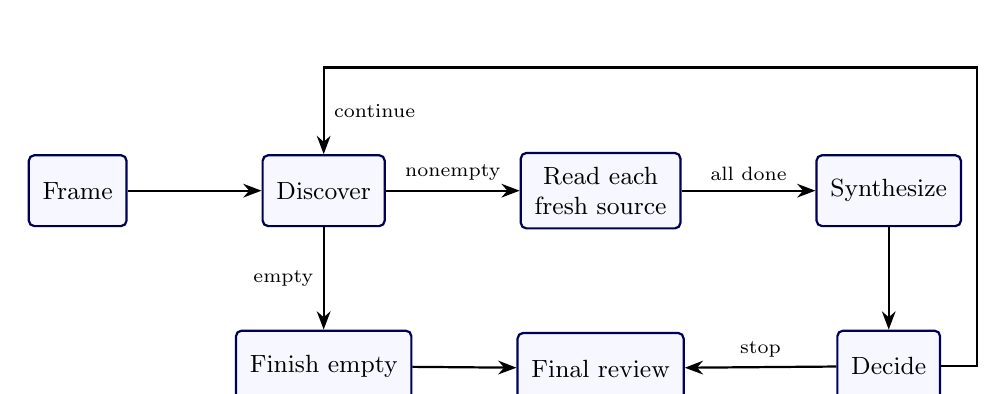
\begin{tikzpicture}[>=Stealth,node distance=9mm and 17mm,
  box/.style={draw=blue!35!black,rounded corners=2pt,fill=blue!3,
  align=center,font=\small,minimum height=9mm,inner sep=5pt},
  every path/.style={thick}]
\node[box] (frame) {Frame};
\node[box,right=of frame] (discover) {Discover};
\node[box,right=of discover] (read) {Read each\\fresh source};
\node[box,right=of read] (synth) {Synthesize};
\node[box,below=13mm of synth] (decide) {Decide};
\node[box,below=13mm of discover] (empty) {Finish empty};
\node[box,below=13mm of read] (report) {Final review};
\draw[->] (frame) -- (discover);
\draw[->] (discover) -- node[above,font=\scriptsize]{nonempty} (read);
\draw[->] (read) -- node[above,font=\scriptsize]{all done} (synth);
\draw[->] (synth) -- (decide);
\draw[->] (discover) -- node[left,font=\scriptsize]{empty} (empty);
\draw[->] (empty) -- (report);
\draw[->] (decide) -- node[above,font=\scriptsize]{stop} (report);
\draw[->] (decide.east) -- ++(0.45,0) |- ([yshift=11mm]discover.north) -- node[right,font=\scriptsize]{continue} (discover.north);
\end{tikzpicture}
\end{center}

\subsection{State and handoffs}
A \texttt{State} contains \texttt{question}, \texttt{scope}, \texttt{round}, \texttt{queries}, \texttt{seen}, \texttt{assessments}, and \texttt{synthesis}. It starts at round 1 with empty evidence. Each source contains \texttt{id}, \texttt{url}, and \texttt{title}; its assessment adds \texttt{summary}, \texttt{limitations}, and citation URLs. The appendix \emph{Shared prompts, schemas, and fixture data} in \emph{Finite Agent Machines} supplies the complete schemas; their source is \file{shared/schemas.json} in this document's directory.

Synthesis receives prior state, the current discovery result, and exactly the current batch of assessments. Before deciding, the process appends the current URLs and assessments to state and replaces its cumulative synthesis. Continuing increments the round and replaces the query list; it preserves the question, scope, and accumulated evidence. A report belongs to the stop route, including the separate empty-discovery route.

There is no authored number of readers or review rounds. Resource and runtime limits can still stop an execution. An operation crash is a failure, not an empty assessment: synthesis must not consume a partial batch. A source that cannot be accessed is different; its reader can succeed with an explicit statement of that limitation. The process does not guarantee eventual convergence, exhaustive coverage, or the quality of its findings.

\subsection{Meaning of ``the same process''}
The definitions share canonical domain instructions, intended response shapes, state transitions, branch conditions, and test fixtures. The three programmatic examples consume the canonical JSON schemas; the Alinery Playbook describes the fields in its agent instructions and does not load or validate those schemas. They do not share a scheduler. Each system applies its own native execution mechanism where tested. Tool permissions, agent context, serialization, persistence, and error handling are not identical. In particular, the Alinery engine treats artifact contents as opaque; semantic conditions such as source identity and exclusive branch publication are agent instructions here. The other examples include host-language response guards. This is a comparison of a matched intended process, not a proof of identical behavior for every invalid output.

\section{How the four definitions express the process}
\subsection{Claude Code Dynamic Workflows}
The saved script uses ordinary JavaScript state, a \texttt{while} loop, and \texttt{pipeline(sources, ...)} to invoke one native \texttt{agent} per discovery result. Awaiting the pipeline supplies the join before synthesis. A returned decision controls the next iteration. The complete script is generated by embedding the common prompts and schemas because the workflow environment does not load modules or directly access the filesystem. It runs separately from the supervising conversation. This is a direct example of dynamic process-driven execution: a fixed script can create a changing number of subagent invocations at runtime.\cite{claude-workflows}

\subsection{Smithers flows}
Smithers calls its authored units \emph{flows}. This example uses its current typed \texttt{Action}, \texttt{Flow}, \texttt{Node}, \texttt{Interpreter}, and \texttt{FlowEngine} APIs. Discovery hands off to a round whose payload supplies the source list. The round constructs one reader action per source and joins them with \texttt{Node.all}. A decision selects a branch that returns the report or hands off to discovery again. The plan can therefore change between rounds while the flow definitions remain fixed.\cite{smithers-bodies,smithers-rounds}

The comparison uses the latest source snapshot inspected for this draft, whose packages identify themselves as 1.0.0-rc.1. It uses the actual in-memory engine and unmodified upstream source. A resolver is included because these packages were not published for direct installation at the inspected revision. The example does not demonstrate durable recovery or cross-process replay; it does not need those features to demonstrate dynamic process control.

\subsection{LangGraph}
The graph defines the six operations once. Discovery returns a list of native \texttt{Send} objects, each carrying a source and the current state to the reader node. LangGraph runs these readers in a super-step; the following super-step reaches synthesis after all readers succeed. A reducer collects tagged assessments, and synthesis selects the current round. Conditional edges handle both the empty discovery and the continue/stop decision. The number of node invocations varies although the node definitions are fixed. This uses LangGraph's graph and super-step semantics, rather than an LLM supervisor deciding every launch.\cite{langgraph-api,langgraph-pregel}

\subsection{Alinery Playbook (FAM)}
The Playbook declares six agent operations and their artifact selectors. Discovery publishes either a batch and one source-request file per fresh source, or an empty disposition. The reader's \texttt{each} input makes each request eligible for its own execution. Synthesis's \texttt{complete} input waits for the corresponding assessment collection. A continuing decision publishes a new occurrence of the round-request artifact, enabling discovery again; stopping publishes the review. The engine tracks artifact occurrences and their provenance, so a repeated logical name does not mean ``read the newest matching file.''\cite{alinery-source}

Here the process is visible in a TOML-and-Markdown document containing prompts and artifact bindings. This representation limits what the engine interprets: it schedules from accepted artifact handoffs, while agents interpret content and choose which output route to publish. A reader can inspect the process without following general-purpose routing functions, but must still understand the selector semantics and prompt obligations. Whether that tradeoff improves review and maintenance is a concrete question this example can support, not a result established by its existence.

\section{Verification and reproducibility}
\subsection{Versions and evidence boundaries}
\begin{tabularx}{\linewidth}{@{}>{\raggedright\arraybackslash}p{0.16\linewidth}>{\raggedright\arraybackslash}p{0.23\linewidth}X@{}}
\toprule
System & Snapshot & Verification performed \\
\midrule
Claude Code & CLI 2.1.289 & 11 Node compatibility checks. \textbf{Native workflow runtime and live inference unverified.} \\
Smithers & 1.0.0-rc.1; source \texttt{8fee1a6d88ef} & 13 checks on the native in-memory engine, with fixture agent results. \\
LangGraph & 1.2.14; Python 3.14.5 & 11 checks on the installed native graph runtime, plus a fixture CLI run. \\
Alinery & Whitepaper snapshot \texttt{d9768d9a8dbe}; core 0.20.1 & 6 checks using production parsing, scheduling, reservation, completion, and exit-confirmation code. Agent outputs and lifecycle signals simulated. \\
\bottomrule
\end{tabularx}

The pinned Smithers commit is \file{8fee1a6d88ef0308159cb1c9bd6a462ebf660724}; its example pins Node 26.4.0 and Effect 4.0.0-rc.115. The Alinery snapshot is \file{d9768d9a8dbea228860e2a4408f7079a5952e788}. Its core source tree is \file{8155b475cf4179cb93eea45102e3d69cdc41e172}. Dependency locks and machine-readable evidence are included in the source bundle. These are point-in-time pins, not claims about future releases.

The normal fixture discovers A and B, waits for both readers, synthesizes, continues, discovers C, and stops after a second synthesis and decision. Other checks cover empty first and second rounds, a failed reader, a single reader, and duplicate URLs. Additional malformed-response checks differ by implementation and should not be interpreted as comparative test scores. Every fixture finding is marked \texttt{SIMULATED}, and every fixture paper URL uses \texttt{example.invalid}.

Smithers and LangGraph evidence records overlapping readers and the barrier before synthesis. Alinery verifies that readers are jointly eligible with widths 2 then 1; its boundary driver completes them sequentially. It also verifies that accepted producer outputs are not released downstream before confirmed process exit. The Claude harness supplies \texttt{agent} and \texttt{pipeline} shims, so it checks script logic but cannot establish native scheduling, permission handling, checkpointing, or replay.

\subsection{What remains unverified}
The installed Claude CLI was signed out. Consequently neither the native Claude workflow nor any live Claude adapter was run. Alinery's desktop app, daemon, PTYs, OMP, and live models were not launched. Its fixture driver exercises core scheduling rather than the complete product. The repository-wide check was attempted but stopped because \file{alinery-app/node_modules} was absent. None of these gaps is hidden by the successful fixture checks.

The live adapters for Smithers and LangGraph launch a fresh Claude CLI process for each operation. They use the same phase instructions and output schemas, but their tool and system-prompt configuration differs; the Alinery example uses the selected OMP configuration. No comparison of model quality, cost, latency, or reproducibility across models is made. Native authenticated runs and inspection of their outputs are still required before treating these as demonstrated end-to-end literature reviews.

\subsection{Where to find the implementation examples}
The implementation appendices have moved to
\href{../playbook-execution-model/v3/playbook-execution-model.pdf}{\emph{Finite Agent Machines}}:
\emph{Claude Code Dynamic Workflow}, \emph{Smithers flow}, \emph{LangGraph graph},
and \emph{Alinery Playbook (FAM)}, followed by
\emph{Shared prompts, schemas, and fixture data}. They contain the complete
process sources and the authored helpers required for their live entry points.
The executable files, dependency locks, test drivers, detailed evidence, and
expanded launch instructions remain in this document's source directory.
Preserve the sibling implementation and \file{shared/} directories.

Claude's appendix prints the complete body and generator, rather than
duplicating the embedded shared constants. Running the generator creates the
self-contained workflow script in the bundle. The Alinery appendix prints its
complete generated Playbook, which runs without a generator. The Smithers and
LangGraph appendices contain their complete live entry points; no omitted
helper implements their branching or looping. The source bundle includes the
whitepaper's source and reading PDF alongside this comparison.

\begin{thebibliography}{9}
\bibitem{claude-workflows} Anthropic. \emph{Dynamic workflows}. \url{https://code.claude.com/docs/en/workflows}. Accessed 7 October 2026.
\bibitem{claude-cli} Anthropic. \emph{Claude Code CLI reference}. \url{https://code.claude.com/docs/en/cli-reference}. Accessed 7 October 2026.
\bibitem{smithers-bodies} Smithers. \emph{Bodies and plans}. Source at commit \texttt{8fee1a6d88ef}. \url{https://github.com/smithersai/smithers/blob/8fee1a6d88ef0308159cb1c9bd6a462ebf660724/packages/smithers/flows/flow/docs/concepts/bodies-and-plans.md}.
\bibitem{smithers-rounds} Smithers. \emph{Trampoline rounds}. Same commit. \url{https://github.com/smithersai/smithers/blob/8fee1a6d88ef0308159cb1c9bd6a462ebf660724/packages/smithers/flows/flow/docs/concepts/trampoline-rounds.md}.
\bibitem{langgraph-api} LangChain. \emph{Graph API overview}. \url{https://docs.langchain.com/oss/python/langgraph/graph-api}. Accessed 7 October 2026.
\bibitem{langgraph-pregel} LangChain. \emph{Pregel runtime}. \url{https://docs.langchain.com/oss/python/langgraph/pregel}. Accessed 7 October 2026.
\bibitem{alinery-source} Alinery. \emph{Playbook parser, scheduler, and execution state}. Whitepaper source snapshot. \url{https://github.com/DeleganceAI/alinery/tree/d9768d9a8dbea228860e2a4408f7079a5952e788/alinery-app/src-tauri/alinery-core/src}.
\end{thebibliography}

\end{document}
